\section{Realisierung flache FSM}

\subsection{Mögliche Realisierungen von flachen FSMs}

\begin{outline}
    \1 Steuerkonstrukt (typischerweise mit \textbf{switch-case})
        \2 prozedural oder objektorientiert
    \1 Definition und Abarbeitung einer \textbf{Tabelle}
        \2 prozedural oder objektorientiert
    \1 \textbf{State Pattern} (Gang of Four, GoF)
        \2 nur objektorientiert
    \1 Generisch mit Templates
        \2 nur mit einer Sprache, die Templates unterstützt (z.B. C++)
\end{outline}

\vspace{0.2cm}

Jede hierarchische FSM kann in eine flache FSM umgewandelt werden.
\vspace{0.1cm}

\textrightarrow\ Alle Varianten haben wie immer sowohl Vor- als auch Nachteile \\
\textrightarrow\ Bei allen Varianten sind auch Variationen vorhanden


\subsection{Realisieurng mit Steuerkonstrukt (prozedural in C)}

\subsubsection{State-Event-Diagram -- Up/Down-Counter}

\begin{center}
    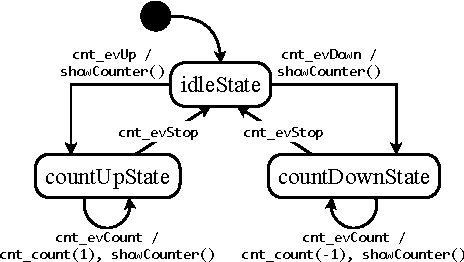
\includegraphics[width=0.8\columnwidth]{images/fsm_up-down-counter_diagramm_C.pdf}
\end{center}

\columnbreak


\subsubsection{Implementation der Prozeduralen Realisierung in C}

\begin{outline}
    \1 \textbf{Ereignisse (events)}
        \2 Schnittstelle nach aussen \textrightarrow\ ändern Zustand der FSM
        \2 In enum definiert (\textbf{public}) \textrightarrow\ header-file
        \2 Einzelne Events und enum Bezeichnung enthalten \textbf{Unitkürzel} (hier: \mylstbox{cnt_})
    \1 \textbf{Zustände (states)}
        \2 In enum definiert (\textbf{nicht} public) \textrightarrow\ sourcecode-file
    \1 \textbf{Aktueller Zustand} wird in einer \textbf{statischen Varianlen} gehalten
    \1 Die FSM wird in \textbf{zwei Funktionen} implementiert
        \2 Initialiserungs-Funktion (hier: \mylstbox[morekeywords={[3], initValue}]{void cnt_ctrlInit(int initValue)})
        \2 Prozess-Funktion (hier: \mylstbox[morekeywords={[3], e}]{void cnt_ctrlProcess(cnt_Event e)}) \\
            \textrightarrow\ Zustände prüfen, Zustandsübergänge veranlassen
    \1 Anstossen einer FSM
        \2 Initialisierung in \lstinline|main|-Funktion
        \2 Überprüfung, welches Event aufgetreten ist meist in \mylstbox{do-while}-Schleife
\end{outline}


\subsubsection{Eigenschaften der Prozeduralen Realisierung in C}

\begin{outline}
    \1 Da aktueller Zustand eine statische Variable ist, kann es nur \textbf{eine einzige Instanz} der FSM geben
    \1 Bei mehreren Instanzen in C...
        \2 darf \mylstbox[morekeywords={[3], currentState}]{currentState} nicht \mylstbox{static} sein und muss als Parameter mitgegenen werden,
            bzw. ein Pointer auf die jeweilige Variable
        \2 Zustands-enum muss in die Schnittstelle (header-file) oder es muss z.B. mit \mylstbox{void*} gearbeitet werden
    \1 In C ist \textbf{keine schöne Kapselung} der Attribute möglich (\mylstbox[morekeywords={[3], currentState}]{currentState})
    \1 Funktion \mylstbox{cnt_ctrlProcess()} kann beliebig aufgerufen werden (periodischer Task, laufend, etc.)
    \1 Bei exponierten Funktionen / Definitionen muss in C ein Unitkürzel vorangestellt werden (hier: \mylstbox{cnt_})
\end{outline}


\example{Up/Down-Counter (prozedural in C)}

\begin{minipage}[t]{0.48\columnwidth}
    \para{Schnittstelle Counter} 
    \lstinputlisting[aboveskip=1mm, belowskip=0mm, morekeywords={[3], val, step}]{snippets/fsm_procedural_C/fsm_counter_C.h}
\end{minipage}
\hfill
\begin{minipage}[t]{0.48\columnwidth}
    \para{Implementation Counter} 
    \lstinputlisting[aboveskip=1mm, belowskip=0mm, morekeywords={[3], val, step, countValue}]{snippets/fsm_procedural_C/fsm_counter_C.c}
\end{minipage}


\para{Schnittstelle FSM} 
\lstinputlisting[aboveskip=1mm, belowskip=0mm, morekeywords={[3], initValue, e}, morekeywords={[2], cnt_Event}]{snippets/fsm_procedural_C/fsm_counterCtrl_C.h} 

\para{Implementation FSM} 
\lstinputlisting[aboveskip=1mm, belowskip=0mm, lastline=19,
                 morekeywords={[3], currentState, initValue, e}, morekeywords={[2], State, cnt_Event}]
                {snippets/fsm_procedural_C/fsm_counterCtrl_C.c}

\columnbreak

\lstinputlisting[aboveskip=0mm, belowskip=0mm, firstline=21, firstnumber=21,
                 morekeywords={[3], currentState, initValue, e}, morekeywords={[2], State, cnt_Event}]
                {snippets/fsm_procedural_C/fsm_counterCtrl_C.c}

\para{Anstossen der FSM} 
\lstinputlisting[aboveskip=1mm, belowskip=0mm, morekeywords={[3], answer}]{snippets/fsm_procedural_C/fsm_main_counterTest_C.c}



\subsection{Realisieurng mit Steuerkonstrukt (objektorientiert in C++)}
\label{Realisieurng mit Steuerkonstrukt (objektorientiert in CPP)}

\subsubsection{State-Event-Diagram -- Up/Down-Counter}
\label{State-Event-Diagram -- Up/Down-Counter in CPP}

\begin{center}
    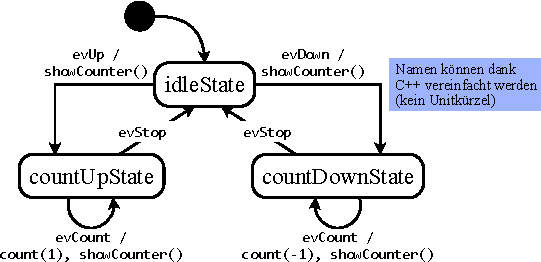
\includegraphics[width=0.8\columnwidth]{images/fsm_up-down-counter_diagramm_CPP.pdf}
\end{center}


\subsubsection{Zusammenhang der Klassen Counter und CounterCtrl}
\label{Zusammenhang der Klassen Counter und CounterCtrl}

\begin{center}
    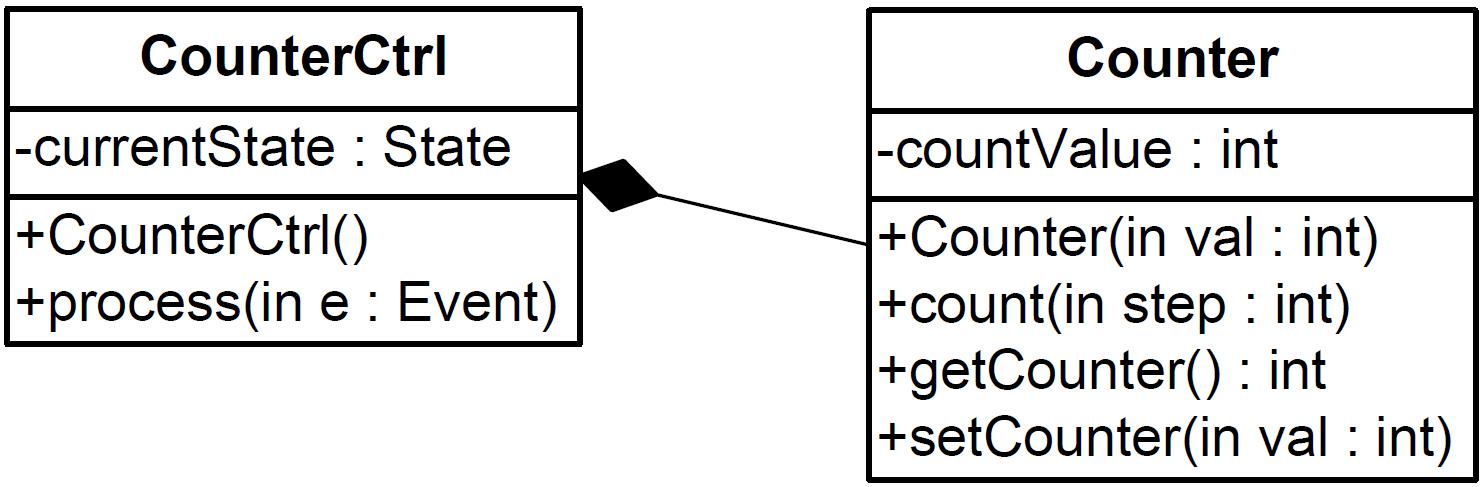
\includegraphics[width=0.7\columnwidth]{images/fsm_CPP_klassendiagramm.png}
\end{center}

\begin{outline}
    \1 Klasse \mylstbox{Counter} führt eigentliche Rechenaufgaben durch
        \2 ist bei \textbf{allen} (objektorientierten) Realiseurngsarten \textbf{identisch}
    \1 Klasse \mylstbox{CounterCtrl} ist FSM, welche Zugriff auf den Counter steuert 
\end{outline}

\textbf{ \textrightarrow\ Generell sollten Steuerung und Element, das gesteuert wird, getrennt werden!}


\subsubsection{Implementation der Prozeduralen Realisierung in C++}

\begin{outline}
    \1 \textbf{Ereignisse (events)}
        \2 Schnittstelle nach aussen \textrightarrow\ ändern Zustand der FSM
        \2 Im \textbf{public} Teil der Klasse als enum definiert
        \2 Keine Unitkürzel nötig
    \1 \textbf{Zustände (states)}
        \2 Im \textbf{private} Teil der Klasse als enum definiert \textrightarrow\ header-file
    \1 \textbf{Aktueller Zustand} \mylstbox{currentState} wird in \textbf{privatem Attribut} der Schnittstelle gehalten
    \1 Die FSM wird in \textbf{zwei Funktionen} implementiert
        \2 Kontruktor (hier: \mylstbox[morekeywords={[3], initValue}]{CounterCtrl::CounterCtrl(int initValue=0)})
        \2 Prozess-Funktion (hier: \mylstbox[morekeywords={[3], e}]{void CounterCtrl::process(CounterCtrl::Event e)}) \\
            \textrightarrow\ Zustände prüfen, Zustandsübergänge veranlassen
    \1 Anstossen einer FSM
        \2 Initialisierung in \lstinline|main|-Funktion
        \2 Überprüfung, welches Event aufgetreten ist meist in \mylstbox{do-while}-Schleife
\end{outline}


\example{Up/Down-Counter (prozedural in C++)}

\begin{minipage}[t]{0.44\columnwidth}
    \para{Schnittstelle Counter} 
    \lstinputlisting[aboveskip=1mm, belowskip=0mm, morekeywords={[3], val, step, countValue}]{snippets/fsm_procedural_CPP/fsm_Counter_CPP.h}
\end{minipage}
\hfill
\begin{minipage}[t]{0.52\columnwidth}
    \para{Implementation Counter} 
    \lstinputlisting[aboveskip=1mm, belowskip=0mm, morekeywords={[3], val, step, countValue}]{snippets/fsm_procedural_CPP/fsm_Counter_CPP.cpp}
\end{minipage}


\para{Schnittstelle FSM} 
\lstinputlisting[aboveskip=1mm, belowskip=0mm, lastline=20, morekeywords={[3], initValue, e, myCounter, currentState}, morekeywords={[2], Event, State, Counter}]{snippets/fsm_procedural_CPP/fsm_CounterCtrl_CPP.h} 
\columnbreak
\lstinputlisting[aboveskip=0mm, belowskip=0mm, firstline=22, firstnumber=22, morekeywords={[3], initValue, e, myCounter, currentState}, morekeywords={[2], Event, State, Counter}]{snippets/fsm_procedural_CPP/fsm_CounterCtrl_CPP.h} 

\para{Implementation FSM} 
\lstinputlisting[aboveskip=1mm, belowskip=0mm, morekeywords={[3], initValue, e, myCounter, currentState}, morekeywords={[2], Event, State, Counter}]{snippets/fsm_procedural_CPP/fsm_CounterCtrl_CPP.cpp}
% \lstinputlisting[aboveskip=0mm, belowskip=0mm, firstline=29, firstline=29, morekeywords={[3], initValue, e, myCounter, currentState}, morekeywords={[2], Event, State, Counter}]{snippets/fsm_procedural_CPP/fsm_CounterCtrl_CPP.cpp}


\para{Anstossen der FSM} 
\lstinputlisting[aboveskip=1mm, belowskip=0mm, morekeywords={[3], answer, myFSM}, morekeywords={[2], CounterCtrl}]{snippets/fsm_procedural_CPP/fsm_main_counterTest_CPP.cpp}


\subsection{Realisierung mit Tabelle}

\subsubsection{State-Event-Diagram -- Up/Down-Counter}

Siehe Abschnitt \ref{State-Event-Diagram -- Up/Down-Counter in CPP}


\subsubsection{FSM in Tabellenform}

Das State-Event-Diagramm wird in eine Tabelle 'übersetzt'. \textbf{Jede Zeile der Tabelle entspricht einer Transition (Pfeil) im 
State-Event-Diagramm}

\begin{center}
    \begin{tabular}{llll}
        \toprule
        \textbf{Current State}                  & \textbf{Event}        & \textbf{Action}                   & \textbf{Next State}       \\
        \midrule
        \rowcolor{gray!40} idleState            & evUp                  & showCounter()                     & countUpState              \\
        idleState                               & evDown                & showCounter()                     & countDownState            \\
        \rowcolor{gray!40} countUpState         & evCount               & count(1); showCounter()           & countUpState              \\
        countUpState                            & evStop                & -                                 & idleState                 \\
        \rowcolor{gray!40} countDownState       & evCount               & count(-1); showCounter()          & countDownState            \\
        countDownState                          & evStop                & -                                 & idleState                 \\
        \bottomrule
    \end{tabular}
\end{center}


\subsubsection{Implementation der Realisierung mittels Tabelle in C++}

\begin{outline}
    \1 Die ganze FSM ist in einer Tabelle gespeichert
    \1 \textbf{Aktionen} sind als \textbf{Funktion} implementiert, in der \textbf{Tabelle} steht der entsprichende \textbf{Funktionspointer} % CHECK: sind das Pointer auf Klassenelemente?
    \1 \textbf{Abarbeitung} der FSM erfolgt mittels \textbf{Execution Engine}, die in der Tabelle 'nachschaut', was zu tun ist
        \2 Execution Engine \textbf{ändert sich nicht}, wenn FSM geändert wird!
    \1 \textbf{Transition} wird als klasseninterner \mylstbox{struct} deklariert
        \2 enthält aktuellen Zustand, Event, Funktionspointer auf Aktionsmethode und nächsten Zustand
    \1 \textbf{FSM} wird als statischer, offener Array deklariert
        \2 Hier wird ganze FSM gespeichert
        \2 ein \mylstbox{struct} bildet konkret eine Zeile der Tabelle ab
\end{outline}


\subsubsection{Eigenschaften der Realisierung mittels Tabelle}

\begin{outline}
    \1 Die Tabelle kann prozedural oder \textbf{objektorientiert} implementiert werden
        \2 Objektorientierte Variante verwendet einzig die Datenkapselung (keine Vererbung, kein Polymorphismus)
        \2 Objektorientierte Variante ist klarer / schöner strukturiert
    \1 \textbf{Aktions-Funktionen} können \textbf{nicht inlined} werden, da ein Pointer auf die Funktionen verwendet wird
\end{outline}


\subsubsection{Tabelle vs. prozedural}

\begin{minipage}[t]{0.48\columnwidth}
    \raggedright
    \myul{\textbf{Gemeinsamkeiten}}
    
    \vspace{0.1cm}

    \begin{outline}
        \1 Testprogramm \mylstbox{counterTest.cpp}
        \1 Schnittstelle (public-Teil) von Klasse \mylstbox{CounterCtrl}
        \1 Gesamte Klasse \mylstbox{Counter}
    \end{outline}
\end{minipage}
\hfill
\begin{minipage}[t]{0.48\columnwidth}
    \raggedright
    \myul{\textbf{Unterschiede}}
    
    \vspace{0.1cm}

    \begin{outline}
        \1 private-Teil von Klasse \mylstbox{CounterCtrl} und Implementation davon
    \end{outline}
\end{minipage}


\example{Up/Down-Counter (mit Tabelle in C++)}

\para{Schnittstelle und Implementation von Counter}
Die Schnittstelle \mylstbox{counter.h} und die Implementation \mylstbox{counter.cpp} ändern sich nicht! \\
\textrightarrow\ Code-Beispiele siehe \ref{Realisieurng mit Steuerkonstrukt (objektorientiert in CPP)}

\para{Anstossen der FSM}
Die Implementation des Testprogramms \mylstbox{counterTest.cpp} ändern sich nicht! \\
\textrightarrow\ Code-Beispiele siehe \ref{Realisieurng mit Steuerkonstrukt (objektorientiert in CPP)}

\vspace{0.1cm}

\para{Schnittstelle FSM} 
\lstinputlisting[aboveskip=1mm, belowskip=0mm, lastline=30, morekeywords={[3], initValue, e, myCounter, currentState, ev, pAction, nextState, fsm}, morekeywords={[2], Event, State, Action, Transition, Counter}]{snippets/fsm_table_CPP/fsm_CounterCtrl_table_CPP.h} 
\columnbreak
\lstinputlisting[aboveskip=0mm, belowskip=0mm, firstline=31, firstnumber=31, morekeywords={[3], initValue, e, myCounter, currentState, ev, pAction, nextState, fsm}, morekeywords={[2], Event, State, Action, Transition, Counter}]{snippets/fsm_table_CPP/fsm_CounterCtrl_table_CPP.h} 

\para{Implementation FSM} 
\lstinputlisting[aboveskip=1mm, belowskip=0mm, morekeywords={[3], initValue, e, myCounter, currentState, i, fsm, pAction}, morekeywords={[2], Event, State, Action, Transition}]{snippets/fsm_table_CPP/fsm_CounterCtrl_table_CPP.cpp}


\subsection{Erweiterung der Realisierung mittels Tabellen}

\begin{itemize}
    \item Wenn der Zustandsübergang nicht durch einen Event, sondern eine \textbf{komplexere Prüfung (Event und Guard)} ausgelöst wird, 
        dann könnte der \textbf{Event-Eintrag} in der Tabelle durch einen weiteren \textbf{Funktionspointer} auf eine 
        \textbf{Checkfunktion ersetzt} werden.
    \item Ergänzung für die Behandlung von Entry- und Exit-Actions
\end{itemize}


\example{Up/Down-Counter (mit Checker-Tabelle in C++)}

\begin{outline}
    \1 Änderungen in \mylstbox{CounterCtrl.h} \textrightarrow\ siehe Beispiel-Code
    \1 Änderungen in \mylstbox{CounterCtrl.cpp}
        \2 checker-Funktionen müssen implementiert werden
        \2 In Tabelle steht statt Event die Adresse der checker-Funktion (analog zu action-Funktionen)
\end{outline}

\lstinputlisting[aboveskip=1mm, belowskip=0mm, morekeywords={[3], e, pAction, pChecker, nextState, currentState}, morekeywords={[2], Event, State, Action, Transition, Checker}]{snippets/fsm_table_CPP/fsm_CounterCtrl_table_pChecker_CPP.h}

\columnbreak


\subsection{Realisieurng mit StatePattern}

\subsubsection{Grundidee von StatePatterns}
\label{Grundidee StatePatterns}

Das Grundkonzept von StatePatterns ist \textbf{Polymorphismus} (Vererbung)

\begin{center}
    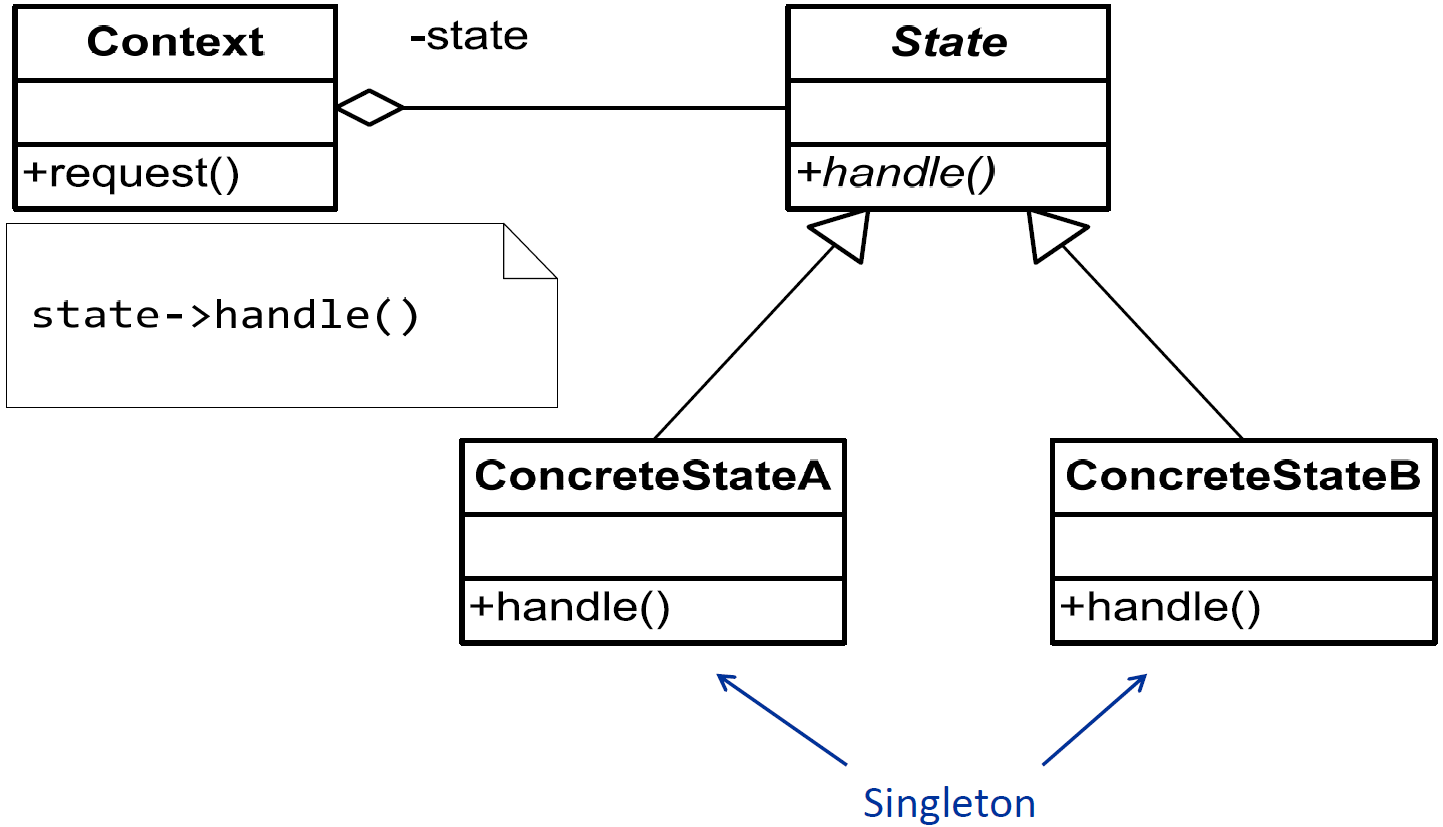
\includegraphics[width=0.8\columnwidth]{images/fsm_state_pattern_struktur.png}
\end{center}

\begin{outline}
    \1 \textbf{Context}-Klasse
        \2 definiert \textbf{Schnittstelle} für Clients
        \2 unterhält eine \textbf{Instanz} einer konkreten Unterklasse von \mylstbox{State}, die den aktuellen Zustand repräsentiert
    \1 \textbf{State}-Klasse
        \2 definiert die Schnittstelle zur FSM in Form einer \textbf{abstrakten Klasse}
    \1 \textbf{ConcreteStateX} Unterklassen
        \2 Jede Unterklasse (Singleton) implementiert genau \textbf{einen Zustand}
\end{outline}


\subsubsection{Transitions in StatePatterns}

StatePattern definiert nicht, wo die Transitions umgesetzt werden sollen. Es gibt daher die zwei folgenden Varianten. \\
\textbf{ \textrightarrow\ Variante 2 ist klar zu bevorzugen!}

\vspace{0.2cm}

\begin{enumerate}
    \item Transitionen könnten in der \mylstbox{Context}-Klasse definiert werden. \\
        Nachteil: dort müsste zentral sehr viel Intelligenz vorhanden sein \\
        Da diese Klasse auch den Zugriff von der Aussenwelt darstellt, sollte sie möglichst schlank sein.
    \item \mylstbox{State}-Klassen \textbf{realisieren ihre Transitionen selbst.} \\
        \textrightarrow\ wir oft mittels \mylstbox{friend}-Deklaration realisiert, was jedoch nicht nötig ist
\end{enumerate}


\subsubsection{State-Event-Diagram -- Up/Down-Counter}
\label{State-Event-Diagram -- Up/Down-Counter - StatePattern}

\begin{center}
    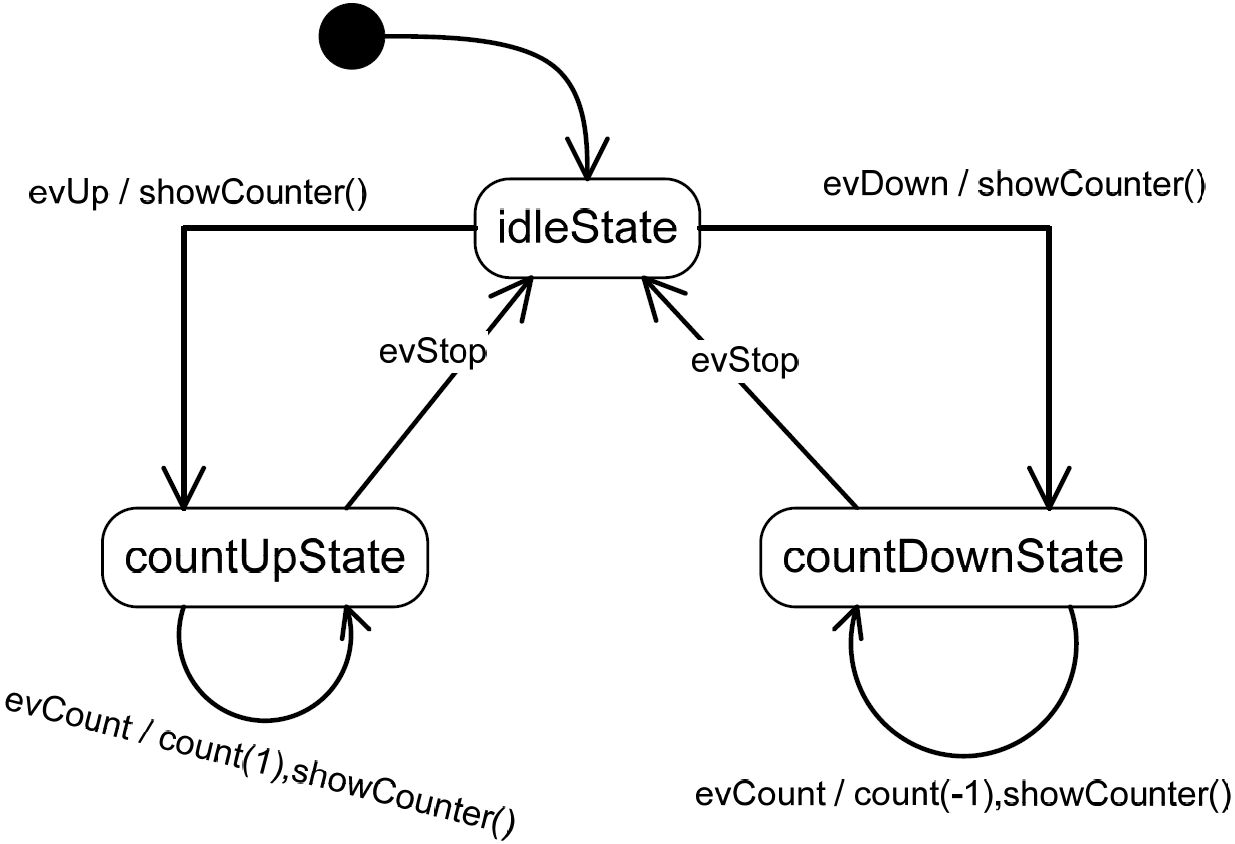
\includegraphics[width=0.75\columnwidth]{images/fsm_up-down-counter_diagramm_state_pattern.png}
\end{center}


% \subsubsection{Klassendiagramm -- Up/Down-Counter}
% \label{Klassendiagramm -- Up/Down-Counter - StatePattern}

% \begin{center}
%     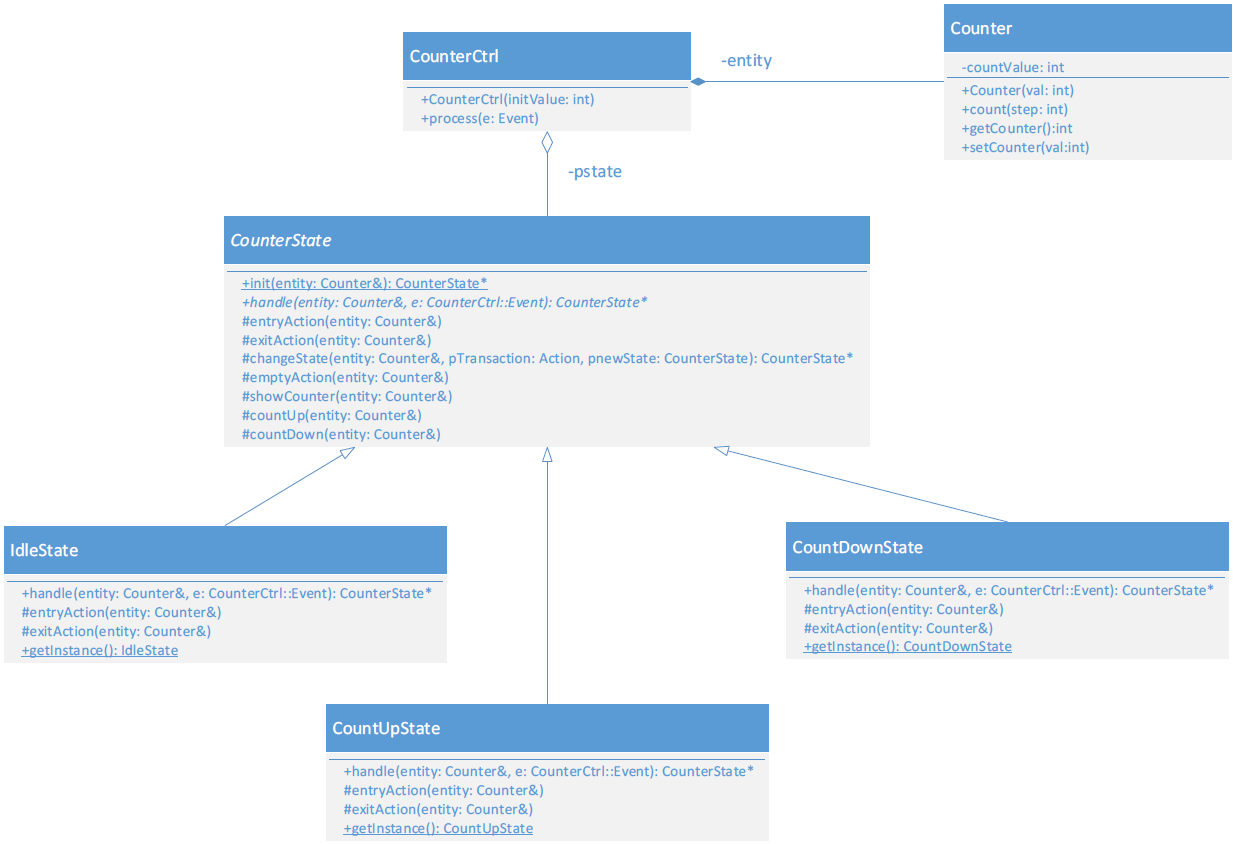
\includegraphics[width=0.95\columnwidth]{images/fsm_up-down-counter_klassendiagramm_state_pattern.png}
% \end{center}


\subsubsection{Implementation der Realisierung mittels StatePattern}

\begin{outline}
    \1 \textbf{Ereignisse (events)}
        \2 Schnittstelle nach aussen \textrightarrow\ ändern Zustand der FSM
        \2 Im \textbf{public} Teil der abstrakten Basisklasse als enum definiert
    \1 \textbf{Zustände (states)}
        \2 Jeder Zustand als eigene (Sub-)Klasse definert
    \1 \textbf{Aktueller Zustand} \mylstbox{pState} wird in \textbf{privatem Attribut (Pointer!)} der Schnittstelle gehalten
        \2 Es braucht daher in der \mylstbox{Context}-Klasse eine \textbf{forward declaration} der \mytclstbox{State}-Klasse
    \1 Die FSM wird in \textbf{zwei Funktionen} implementiert
        \2 Kontruktor (hier: \mylstbox[morekeywords={[3], initValue}]{CounterCtrl::CounterCtrl(int initValue=0)})
        \2 Prozess-Funktion (hier: \mylstbox[morekeywords={[3], e}, morekeywords={[2], Event}]{void CounterCtrl::process(CounterCtrl::Event e)}) \\
            \textrightarrow\ Zustände prüfen, Zustandsübergänge veranlassen
    \1 \textbf{Entry- und Exit-Actions}
        \2 Können in Basisklassen-Methode \mylstbox{changeState()} isoliert vorgenommen werden
        \2 Zwischen Exit- und Entry-Action müssen allfällige Transition-Actions ausgeführt werden. Diese wird in der Methode 
            \mylstbox{changeState()} als \textbf{Funktionspointer} übergeben
        \2 In Basisklasse werden zwei \textbf{virtuelle Methoden} \mylstbox{entryAction()} und \mylstbox{exitAction()} deklariert \\
            \textrightarrow\ Default-Implementation sinnvoll!
\end{outline}


\example{Up/Down-Counter mit StatePattern}


\para{Schnittstelle und Implementation von Counter}

Die Schnittstelle \mylstbox{counter.h} und die Implementation \mylstbox{counter.cpp} ändern sich nicht! \\
\textrightarrow\ Code-Beispiele siehe \ref{Realisieurng mit Steuerkonstrukt (objektorientiert in CPP)}

%TODO: check includes for every file...
\para{Schnittstelle zur FSM} 
\lstinputlisting[aboveskip=1mm, belowskip=0mm, morekeywords={[3], initValue, e, entity, pState}, morekeywords={[2], Event, Counter, CounterState}]{snippets/fsm_state_pattern_CPP/fsm_CounterCtrl_state_pattern.h}

\para{Implementation der FSM} 
\lstinputlisting[aboveskip=1mm, belowskip=0mm, morekeywords={[3], initValue, e, entity, pState}, morekeywords={[2], Event, Counter, CounterState}]{snippets/fsm_state_pattern_CPP/fsm_CounterCtrl_state_pattern.cpp}


\para{Schnittstelle abstrakte State-Basisklasse}   
\lstinputlisting[aboveskip=1mm, belowskip=0mm, morekeywords={[3], initValue, e, entity, pState, pnewState, ptransAction, CounterState}, morekeywords={[2], Event, Counter, Action}]{snippets/fsm_state_pattern_CPP/fsm_CounterState_state_pattern.h}

\para{Implementation abstrakte State-Basisklasse}
\lstinputlisting[aboveskip=1mm, belowskip=0mm, morekeywords={[3], initValue, e, entity, pState, initState, pnewState, ptransAction}, morekeywords={[2], Event, Counter, CounterState, Action}]{snippets/fsm_state_pattern_CPP/fsm_CounterState_state_pattern.cpp}

\columnbreak


\para{Schnittstelle ConcreteStateX-Klassen (CountUpState)}
\lstinputlisting[aboveskip=1mm, belowskip=0mm, morekeywords={[3], initValue, e, entity, pState}, morekeywords={[2], Event, Counter, CounterState}]{snippets/fsm_state_pattern_CPP/fsm_ConcreteState.h} 

\para{Implementation ConcreteStateX-Klassen (CountUpState -- no actions)}
\lstinputlisting[%
aboveskip=1mm,
belowskip=0mm,
morekeywords={[3], instance, entity, e}, morekeywords={[2], Event, Counter, CounterState}]
{snippets/fsm_state_pattern_CPP/fsm_ConcreteState.cpp} 

\para{Implementation ConcreteStateX-Klassen (CountUpState -- with actions)}
\lstinputlisting[aboveskip=1mm, belowskip=0mm, morekeywords={[3], instance, entity, e}, morekeywords={[2], Event, Counter, CounterState}]{snippets/fsm_state_pattern_CPP/fsm_ConcreteState_with_actions.cpp} 

\para{Anstossen der FSM}
Die Implementation des Testprogramms \mylstbox{counterTest.cpp} ändern sich nicht! \\
\textrightarrow\ Code-Beispiele siehe \ref{Realisieurng mit Steuerkonstrukt (objektorientiert in CPP)}

